\section{Ladder Operator Block-Encoding (LOBE)}
\label{sec:lobe}

The block-encodings presented in this work builds off of the construction of \cite{liu2024efficient} to provide a more general block-encoding of Hamiltonians described in the form of Eq. \ref{eq:lclo}.
Explicity, the construction presented in this work allows for the terms in the Hamiltonian to be any arbitrary product of ladder operators acting on fermions, antifermions, and bosons.
Additionally, we make use of the observations presented in Subsection \ref{subsec:unification} to provide block-encodings of the same structure as an LCU which have reduced rescaling factors.
This also extends LCU block-encodings to the non-unitary operators used in this work and may provide a framework for constructing block-encodings of linear combinations of other non-unitary operators.

\subsection{Rescaling of Coefficients Due to Bosonic Terms}
\label{subsec:rescaling}

The inclusion of bosonic ladder operators in our models requires rescaling the coefficients of our Hamiltonian such that they are always normalized and appropriately weighted.
As shown in Eqs. \ref{eq:bosonic-creation} and \ref{eq:bosonic-annihilation}, bosonic ladder operators acquire a coefficient on the state that is proportional to the square-root of the occupation of the state.
From these definitions, it is clear that if we were to apply a block-encoding that contains bosonic ladder operators onto a quantum state, the output quantum state may not be normalized.

To remedy this, we can rescale the coefficients that are picked up by the operators such that the states are always normalized.
In the case of bosonic ladder operators, we can rescale Eqs. \ref{eq:bosonic-creation} and \ref{eq:bosonic-annihilation} by dividing by the square-root of the maximum allowable occupation number plus one such that any coefficient acquired is $< 1$:
\begin{equation}
    \label{eq:bosonic-ops-altered}
    \begin{split}
        \Tilde{a}_i^\dagger \ket{n_{a_i}} &= \sqrt{\frac{n_{a_i} + 1}{\Omega + 1}} \ket{n_{a_i} + 1} \hspace{1em} when \ket{n_{a_i}} \neq \ket{\Omega} \\
        \Tilde{a}_i  \ket{n_{a_i}} &= \sqrt{\frac{n_{a_i}}{\Omega + 1}} \ket{n_{a_i} - 1} \hspace{1.7em} when \ket{n_{a_i}} \neq \ket{0}
    \end{split}
\end{equation}
We do not redefine these equations for the cases where the state is annihilated since they will be the same as in Eqs.  \ref{eq:bosonic-creation} and \ref{eq:bosonic-annihilation}
These rescaled coefficients will be accounted for within the action of the $Select$ oracle as described in Subsubsection \ref{subsubsec:select}.

Since multiple bosonic operators may be present within a single term ($T_l$), then the overall coefficient of the output state will be rescaled by a factor of:
\begin{equation}
    \lambda_{k_l} = (\Omega + 1)^{k_l/2}
\end{equation}
where $k_l$ is the number of bosonic operators included in the term $T_l$.

Different terms within the Hamiltonian may have different numbers of bosonic operators and therefore will have differing rescaling coefficients of $\lambda_{k_l}$.
In order to guarantee that this rescaling is consistent across the different terms, we can classically preprocess the coefficients in the Hamiltonian such that after the block-encoding is applied, all output states have the same bosonic rescaling factor.
If we define $K \equiv \max_l{k_l}$, then we can define the preprocessed coeffieints as:
\begin{equation}
    \label{bose coeff rescale}
    \alpha_l \rightarrow \frac{\alpha_l}{(\Omega + 1)^{(K - k_l)/2}} \equiv \tilde{\alpha_l}
\end{equation}
where the coefficients $\tilde{\alpha_l}$ are the rescaled coefficients of the terms.

% This preprocessing means that after the block-encoding is applied, all output states will be rescaled by a coefficient of $(\Omega + 1)^{(K)/2}$.
Therefore, the Hamiltonian with rescaled coefficients is given by:
\begin{equation}
    \tilde{H} = \sum_{l=0}^{L-1} \tilde{\alpha_l} \Tilde{T}_l
\end{equation}
where $\tilde{H}$ is the rescaled Hamiltonian and the bosonic operators are replaced with $\Tilde{a}_i^\dagger$ and $\Tilde{a}_i$ the action defined by Equations \ref{eq:bosonic-ops-altered}, such that $\tilde{T} \equiv T(b_i, b_i^\dagger, d_i, d_i^\dagger, \tilde{a}_i, \tilde{a}_i^\dagger)$.

\subsection{Circuit Construction}
\label{subsec:circuit}

\begin{figure}
    \centering
    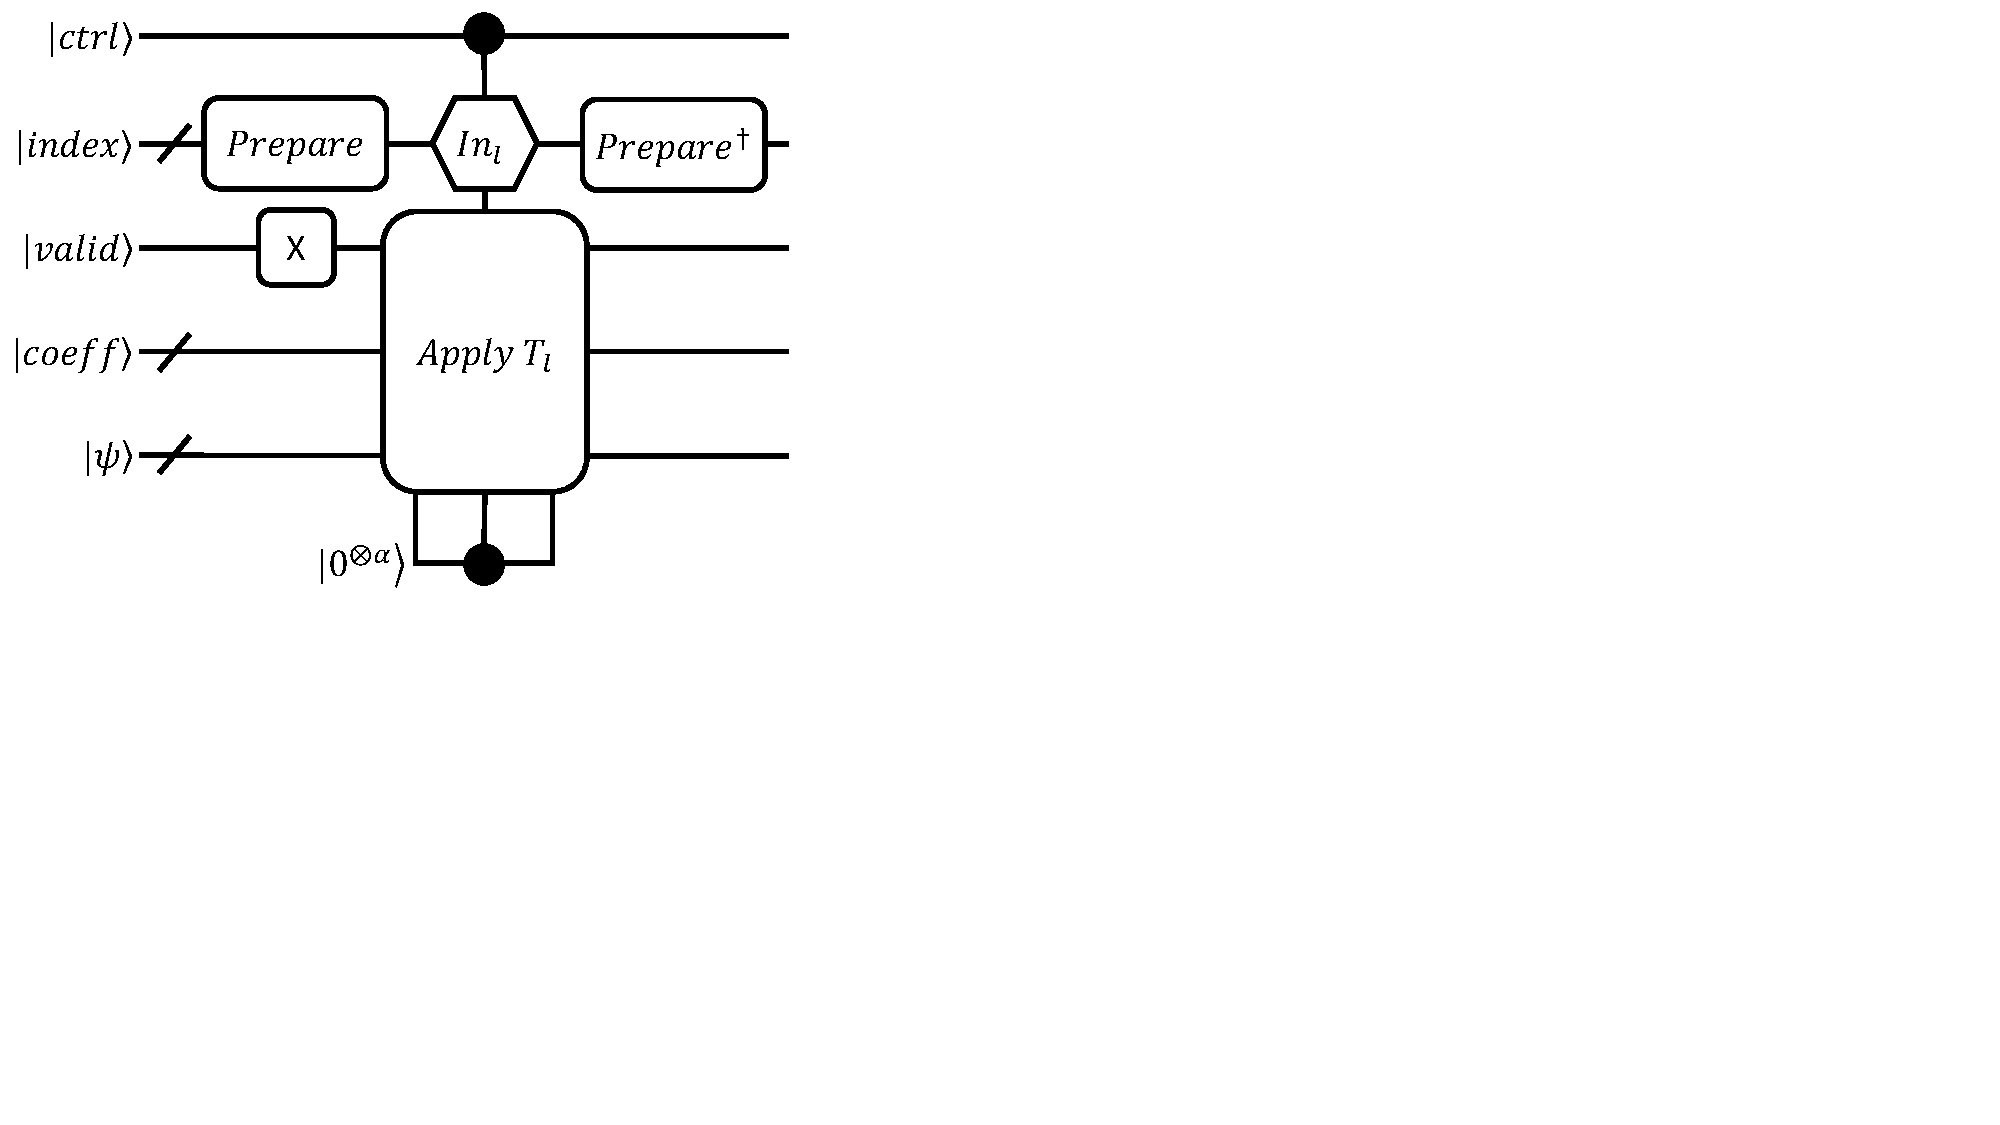
\includegraphics[width=8cm]{figures/lobe-block-encoding.pdf}
    \caption{\textbf{Ladder Operator Block-Encoding.}
    }
    \label{fig:lobe}
\end{figure}

In Figure \ref{fig:lobe}, we define the LOBE circuit in terms of generic oracles.
Disregarding the (optional) control qubit ($\ket{\textit{ctrl}}$), the LOBE circuit makes use of 5 qubit registers: $\ket{\textit{index}}$, $\ket{\textit{valid}}$, $\ket{\textit{coeff}}$, $\ket{\psi}$, and $\ket{0^{\otimes \alpha}}$.

The register denoted $\ket{\textit{index}}$ is referred to as the index register and is used to index the terms in the Hamiltonian as is done in LCU constructions. 
The integer representations of the computational basis states of the index register corresponds to the indices $l$ in Eq. \ref{eq:lclo}. 

The register denoted $\ket{\textit{valid}}$ consists of a single qubit and is referred to as the validation qubit.
It serves the same purpose as in \cite{liu2024efficient} which is to denote whether or not the term at the current index ($T_l$) will annihilate the quantum state.
If the term will annihilate the state, then the validation qubit remains in the $\ket{1}$ state such that the branch of the wavefunction stays outside the desired subspace of the block-encoding.
If the term will not annihilate the state, then the validation qubit gets flipped to the $\ket{0}$ state for the term $T_l$.

The register denoted $\ket{\textit{coeff}}$ is referred to as the coefficient register and is used to apply the coefficients associate with the term $T_l$. 
These coefficients include both the coefficients of the terms in the linear combination ($\alpha_l$) as well as the coefficients associated with the bosonic ladder operators.
One qubit is used to apply the $\alpha_l$ coefficient while a separate qubit will be required for each bosonic operator (defined as a creation, annihilation, or occupation operator acting with a positive integer-valued exponent) in the term.

The register denoted $\ket{\psi}$ is referred to as the system register and is used to encode the state of the system.
This register can be broken up into three subsequent registers: the fermionic system $\ket{\psi_b}$, the antifermionic system ($\ket{\psi_d}$), and the bosonic system ($\ket{\psi_a}$).
The encoding studied in this work is outlined in more detail in Subsection \ref{subsec:encoding}.

Finally, the register denoted $\ket{0^{\otimes \alpha}}$ is referred to as the clean ancillae register.
This register includes ancillae qubits that are promised to begin in the $\ket{0}$ state and are returned to this state at the end of the block-encoding circuit.

The LOBE circuit is structured similarly to an LCU circuit in that it involves sequential application of a $\textit{Prepare}$ oracle, a $\textit{Select}$ oracle, and then uncomputing the $\textit{Prepare}$ oracle using the daggered circuit.
In addition to these oracles, a single $X$ gate is applied to the $\ket{\textit{valid}}$ qubit in order to prepare this qubit in the $\ket{1}$ state.
This single $X$ gate is \textit{not} repeated on subsequent applications of the block-encoding.

\subsubsection{Prepare Oracle}
\label{subsec:prepare-oracle}

The $\textit{Prepare}$ oracle is applied to the index register to prepare a superposition over the computational basis states of this register.

\textbf{Uniform State Preparation}

The simplest implementation of the $\textit{Prepare}$ oracle is to prepare a uniform superposition over the computational basis states using a series of Hadamard gates on each qubit in the register.
The rescaling condition for this implementation is that the coefficients must be rescaled such that they all have magnitude $\leq 1$.
Let the largest coefficient magnitude be given by $\alpha^* = \max{|\tilde{\alpha_l}|}$.
Then, this rescaling imposes a constant rescaling factor of $\alpha^*$ and we refer to these rescaled coeffifients as $\Tilde{\alpha_l}$.
An additional rescaling factor of $2^{\lceil \log_2{L} \rceil}$ from the uniform superposition results in an overall rescaling of the Hamiltonian by a constant factor of:
\begin{equation}
    \label{usp scale}
    \lambda_{usp} = 2^{\lceil \log_2{L} \rceil} \alpha^*
\end{equation}
such that the rescaled Hamiltonian is given by:
\begin{equation}
    \label{Hbar scale}
    H^* = \frac{\tilde{H}}{\lambda_{usp}}
\end{equation}

The quantum resource requirements of this implementation of $\textit{Prepare}$ are negligible as no ancillae are required and only Clifford operations (Hadamards) are performed.
However, this implementation of $\textit{Prepare}$ requires that the rescaled coefficients of the terms ($\Tilde{\alpha_l}$) be incorporated within the $\textit{Select}$ oracle which will be described in Subsubsection \ref{subsubsec:select}.

\textbf{Arbitrary State Preparation}

An alternative implementation of $\textit{Prepare}$ is to use the same implementation traditionally used in LCU circuits.
The coefficients are first rescaled by their $L1-norm$:
\begin{equation}
    \label{eq:asp-scale}
    \lambda_{asp} = \sum_{l=0}^{L-1} |\alpha_l|
\end{equation}
and the rescaled Hamiltonian is given by:
\begin{equation}
    H^* = \frac{\tilde{H}}{\lambda_{asp}}
\end{equation}

It should be noted that $\lambda_{asp} \leq \lambda_{usp}$ \ws{with equality when the coefficients of the terms all have equal magnitude (confirm this)} \ws{and give some analytical proof for this bound}.

Then, a state preparation routine is applied that performs the following operation:
\begin{equation}
    \ket{0^{\otimes \lceil \log_2{L} \rceil}} \rightarrow_{\textit{Prepare}} \sum_{l = 0}^{L-1} \sqrt{|\alpha_l| / \lambda_{asp}} \ket{l}
\end{equation}
This results in a weighted superposition over the computational basis states where the squared amplitudes of the basis states are equal to the magnitude of the associated coefficients \gus{from the Hamiltonian}.

For Hamiltonians that have structure among the coefficients of the terms, implementations of the $\textit{Prepare}$ oracle can be constructed that leverage this structure.
In certain cases, this can drastically reduce the cost of $\textit{Prepare}$ such as is done for the Fermi-Hubbard model in \cite{babbush2018encoding}.
However, when a certain structure cannot be assumed, the Grover-Rudolph algorithm from \cite{grover2002creating} gives a formulaic routine to generate these $\textit{Prepare}$ circuits.

Gover-Rudolph requires $L-1$ rotations, with $1$ being uncontrolled and the others controlled.
The total number of left-elbows is given by:
\begin{equation}
    N_{\textit{left-elbow}} = L + 1 
\end{equation}
with an equal number of right-elbows.
The total number of ancillae is given by:
\begin{equation}
    Q_{asp} = \lceil \log_2{L} \rceil - 2
\end{equation}
It should be noted that these ancillae, which will be returned to $\ket{0}$ after the oracle call completes, will likely be reused in the $\textit{Select}$ oracle and therefore will not contribute to the total qubit requirement of the block-encoding.

Overall, after the bosonic coefficient rescaling is applied and one of these $Prepare$ oracle compilations is chosen and the coefficients rescaled again, the overall rescaling of the Hamiltonian that is block-encoded is given by:
\begin{equation}
    \label{eq:post-process}
    H^* = \frac{H}{(\Omega + 1)^{K/2} \lambda}
\end{equation}
with $\lambda$ being either $\lambda_{usp}$ or $\lambda_{asp}$.

\subsubsection{Select Oracle}
\label{subsubsec:select}

\begin{figure}
    \centering
    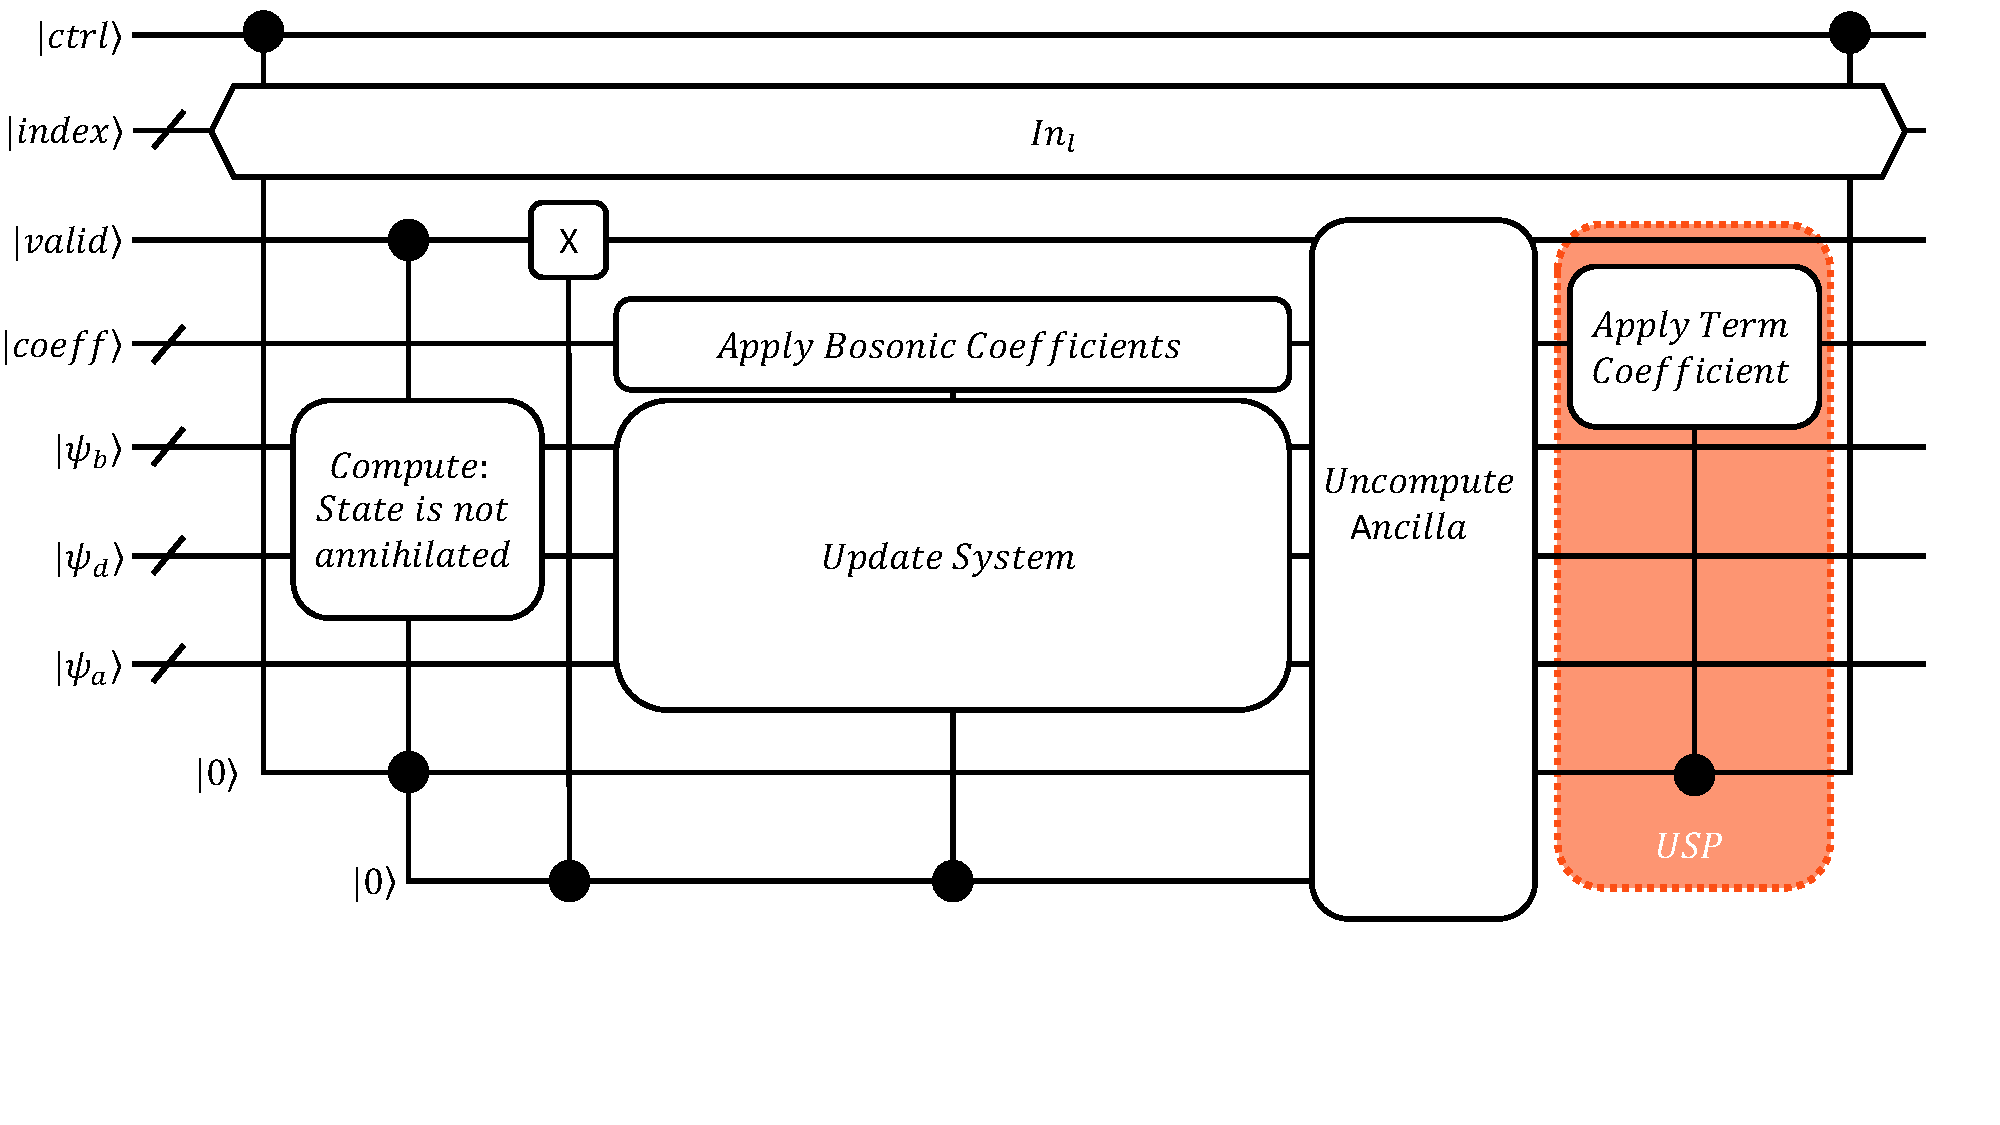
\includegraphics[width=16cm]{figures/select-broad.pdf}
    \caption{\textbf{Ladder Operator Select Oracle.}
    }
    \label{fig:select-broad}
\end{figure}

The $Select$ oracle is shown in Figure \ref{fig:lobe} as the oracle within the blue shaded region.
As is done in standard LCU circuits, the $Select$ oracle is designed such that it applies the term $T_l$ onto the system when the index register is in the computational basis state $\ket{l}$.
In Figure \ref{fig:lobe}, the hexagonal box represents the multiplexing operation given in Figure 7 of \cite{babbush2018encoding} which creates a coherent for-loop over the computational basis states using $L - 1$ left-elbows and $\lceil \log_2{L} \rceil$ ancillae qubits.

In Figure \ref{fig:select-broad}, we depict a broad schematic for applying a single term within the $Select$ oracle in LOBE and in Figure \ref{fig:select} we give a more explicit compilation.
The entire $Select$ oracle can be constructed by applying the circuit for each term ($T_l$) when the ancilla qubit of the multiplexing operator over the index register is in the corresponding computational basis state.

\begin{figure}
    \centering
    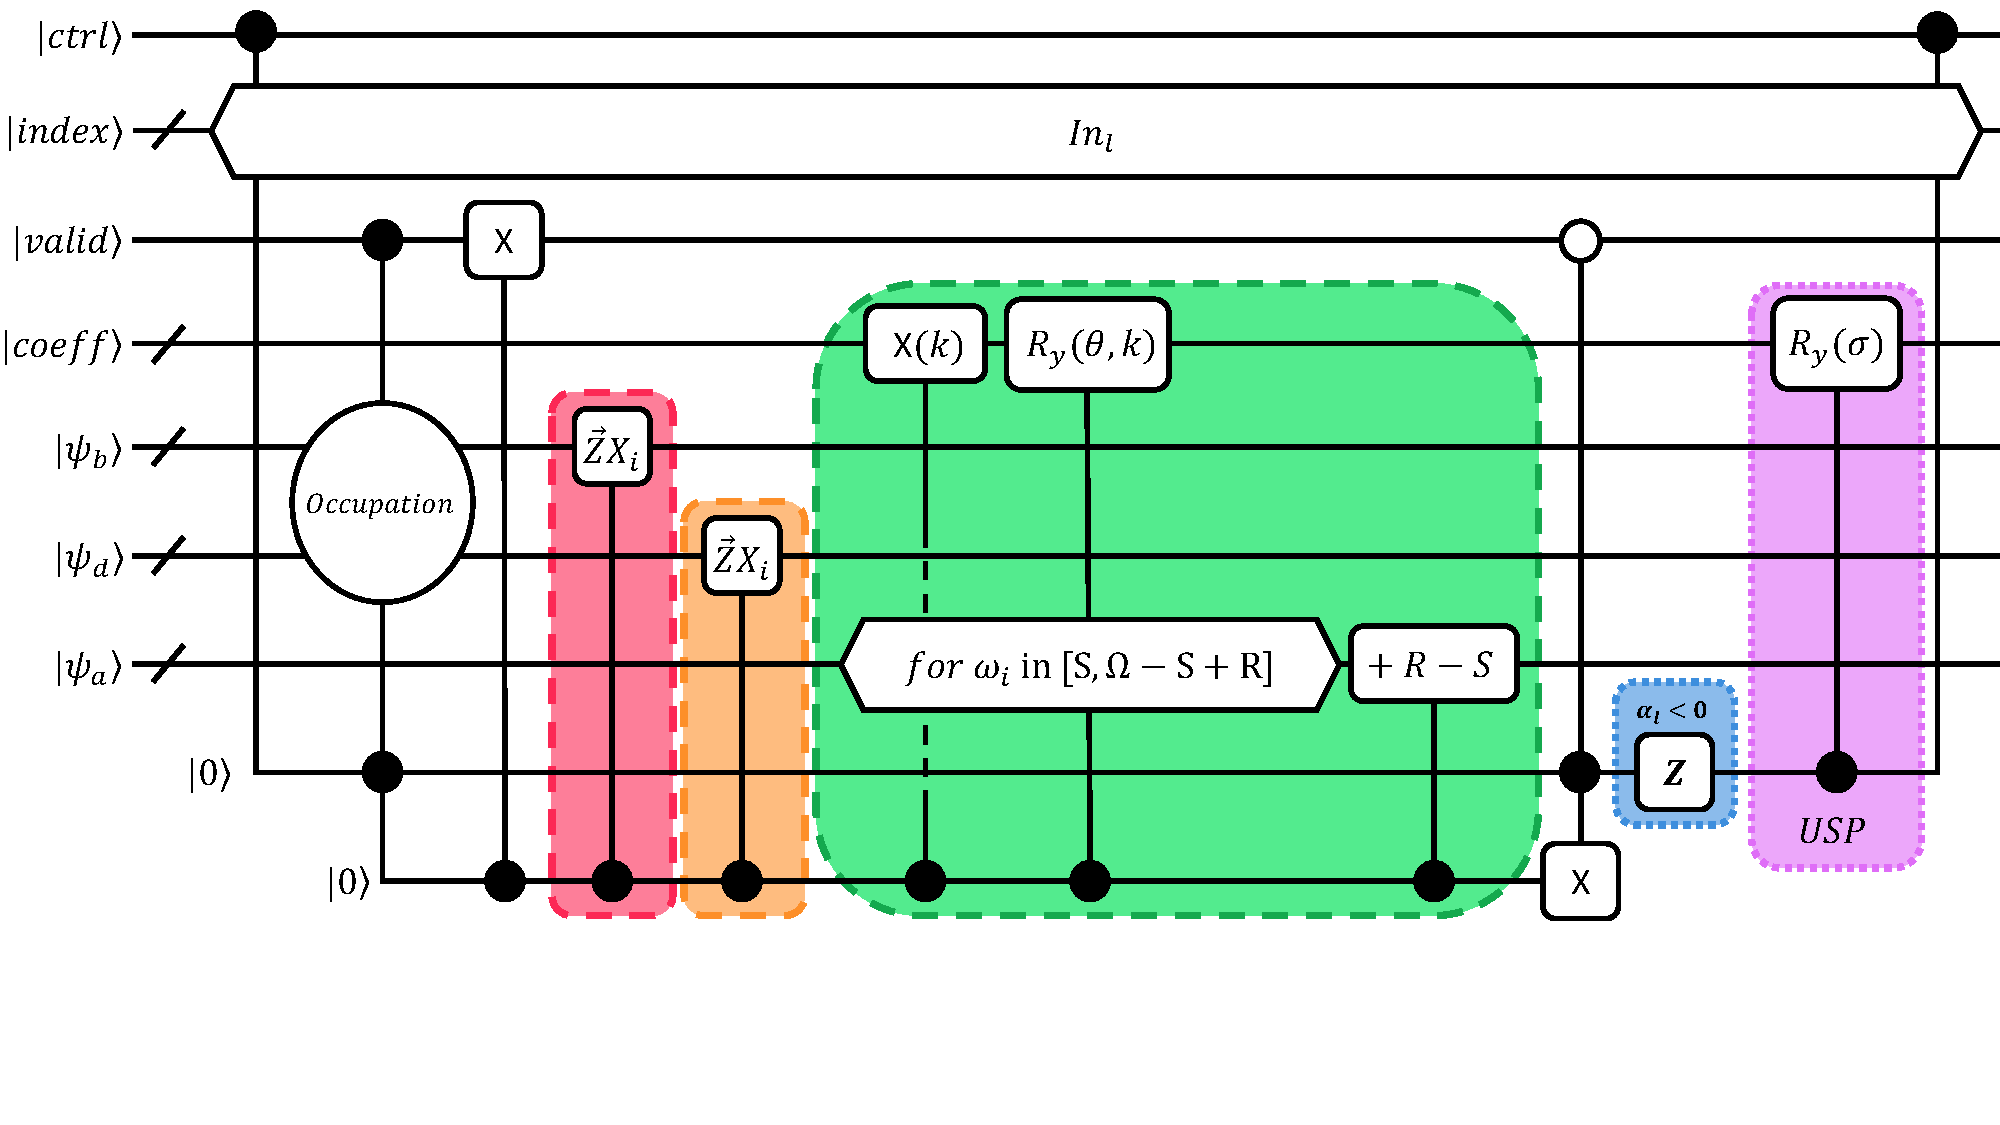
\includegraphics[width=16cm]{figures/select.pdf}
    \caption{\textbf{Ladder Operator Select Oracle (Decomposed).}
    }
    \label{fig:select}
\end{figure}

Working from left to right, the first operation shown in Figure \ref{fig:select} is the left-elbow of the multiplexor which puts the ancilla qubit in the $\ket{1}$ state when the index register is in the computational basis state $\ket{l}$.
Next, a left-elbow - controlled on the validation qubit being in the $\ket{1}$ state, the index register being in the $\ket{l}$ state, and the system being in a state that will not be annihilated - is applied to produce a new ancilla qubit.
To perform a check on if the state will be annihilated, we control based on the occupation of the fermionic and antifermionic modes.
The controls on the fermionic and antifermionic modes are determined by the operators that are present within the current term.
For each fermionic (antifermionic) creation operator acting on mode $i$, a $0$-control is added on $i^{th}$ fermionic (antifermionic) mode within $\ket{\psi_b}$ ($\ket{\psi_d}$).
Likewise, for each fermionic (antifermionic) annihilation operator acting on mode $i$, a $1$-control is added on $i^{th}$ fermionic (antifermionic) mode within $\ket{\psi_b}$ ($\ket{\psi_d}$).
If both ladder operators are present, then only the $1$-control on the $i^{th}$ mode remains since the state gets "zeroed-out" if the mode is unoccupied.
If any of these conditions are not satisfied, then the state should be "zeroed-out" and the ancilla qubit will be in the $\ket{0}$ state for that branch of the wavefunction meaning none of the subsequent operations will be applied.
The quantum states that should be "zeroed-out" due to the bosonic operators will be handled when applying the bosonic operators to the system.

After these checks are performed, the bottom ancilla qubit will be in the $\ket{1}$ state if and only if the three conditions are met, indicating that the term $T_l$ should be applied onto the system.
If the ancilla is in the $\ket{1}$ state, the validation qubit is first flipped from $\ket{1}$ to $\ket{0}$ to put the appropriate branch of the wavefunction into the encoded subspace.
Then the term $T_l$ is applied to the system registers as portrayed in the shaded boxes with the dashed borders in Figure \ref{fig:select}.

In Figure \ref{fig:select}, the first shaded box (red) shows the update on the fermionic system corresponding to a single creation or annihilation operator acting on the $i^{th}$ mode.
Since both the creation and annihilation operators flip the occupation and apply a phase - dependent on the parity of the occupation of the preceeding modes - they can both be applied using the same circuit.
To apply the appropriate phase, Pauli $Z$ gates are applied on all the fermionic modes for $j < i$.
To flip the occupation of the mode that the ladder operator acts on, a Pauli $X$ gate is applied to the $i^{th}$ fermionic qubit.
This series of gates is repeated for all fermionic creation or annihilation operators.
Many of these gates could be compiled out of the circuit, however, they are all Clifford operations and therefore will not significantly contribute to the cost of the block-encoding.
The second shaded box (orange) in Figure \ref{fig:select} portays the application of an antifermionic ladder operator and is constructed in an analogous way, but acts on the corresponding antifermionic modes.

Next, the third shaded box (green) in Figure \ref{fig:select} depicts the action of bosonic ladder operators acting on the $i^{th}$ bosonic mode of the system.
This box is repeated for each bosonic mode that is being acted upon within the current term.
We will define our construction assuming that each term has be normal-ordered, however, we note that the patterns presented here will generalize to terms that are not normal ordered with slight modifications.

Let any series of (normal-ordered) bosonic operators acting on the $i^{th}$ mode be described by:
\begin{equation}
    (a_i^\dagger)^R (a_i)^S
\end{equation}
where $R$ and $S$ are nonzero integers in the range $[0, \Omega]$.

We can describe the action of the rescaled operator on the state of the $i^{th}$ bosonic mode with initial occupation $\omega_i$ as:
\begin{equation}
    \label{eq:bosonic-operator-action}
    (a_i^\dagger)^R (a_i)^S \ket{\omega_i} = \prod_{r=0}^{R-1} \big( \sqrt{\frac{\omega_i - S + r + 1}{\Omega + 1}} \big) \prod_{s=0}^{S-1} \big( \sqrt{\frac{\omega_i - s}{\Omega + 1}} \big) \ket{\omega_i + R - S}
\end{equation}

This operation can implemented in the block-encoding via a quantum circuit as follows with all operations controlled on the ancilla qubit indicating if the current term should be applied, with $k$ denoting the number of bosonic modes that have already been accoutned for in this term:
\begin{enumerate}
    \item Apply a Pauli-X gate on the $k^{th}$ qubit in the coefficient register to rotate it completely outside of the encoded subspace.
    \item Multiplex over the occupation of the $i^{th}$ bosonic mode for occupation states in the range: $S \leq \omega_i \leq \min(\Omega, \Omega - S + R)$. Any state beginning with an occupation less than $S$ will be "zeroed-out" and therefore can be left outside of the encoded subspace without any additional operations. Likewise, any state that should \textit{end} with an occupation greater than $\Omega$ will also be "zeroed-out" and therefore can also be left unmodified.
    \item For each value of $\omega_i$ in the multiplexor, apply a rotation on the $k^{th}$ qubit in the coefficient register of angle $\theta$ given by Eq. \ref{eq:smarter-rot-angle}. The purpose here will be to rotate the qubit back into the encoded subspace with an amplitude in the $\ket{0}$ state equal to the amplitude in Eq. \ref{eq:bosonic-operator-action}. 

    \begin{equation}
        \label{eq:smarter-rot-angle}
        \theta(\omega_i, S, R) = 2 \sin^{-1}{\Big(\prod_{r=0}^{R-1} \big( \sqrt{\frac{\omega_i - S + r + 1}{\Omega + 1}} \big) \prod_{s=0}^{S-1} \big( \sqrt{\frac{\omega_i - s}{\Omega + 1}} \big)\Big)}
    \end{equation}

    \item Update the occupation by a value of $+ R - S$. If $R = S$, no update is needed.
\end{enumerate}

Overall, this requires one multiplexor and one qubit in the coefficient register for each bosonic mode that is being acted upon within the term.
The multiplexors will also have a reduced number of occupation modes to multiplex over, thereby reducing the number of Toffolis required for each multiplexor.

Once the state of the system is updated and the bosonic coefficients have been applied, the bottom ancilla qubit can be uncomputed (reset to $\ket{0}$).
This can be achieved by applying a Toffoli onto this qubit with a zero-control on the validation qubit and a one-control on the ancilla qubit used for multiplexing over the index register.
\ws{It's not quite clear to me if we can use a right-elbow here instead of a Toffoli since we are changing the states of fermionic/antifermionic modes after the left-elbow. Obviously it's only one Toff so it's not a big deal, but I wanna try to do some derivations for this.}

Next, if the sign of the coefficient of the current term is $-1$, we apply a $- \mathds{1}$ - controlled on the index register being in the state $\ket{l}$ - to the state, regardless of which $Prepare$ oracle is used.
This operation is shown in the fourth shaded box (blue) with the dotted border to indicate that this operation may or may not be present depending on the sign of the term.
This can be achieved in many ways, but here we simply use a Pauli-Z gate acting on the ancilla qubit storing the state of the multiplexor acting on the index register.

Finally, if the \textit{uniform state perparation} protocol is used for the $Prepare$ oracle, then a controlled Pauli-Y rotation is applied onto the final qubit in the coefficient register.
This is shown in the fifth shaded box (purple) with the dotted border to indicate that this operation may or may not be present depending on which $Prepare$ oracle is used.
This rotation is used to account for the rescaled coefficient of the term ($\Tilde{\alpha_l}$) and is achieved by applying a rotation with an angle given by:
\begin{equation}
    \sigma(\Tilde{\alpha_l}) \equiv 2 \cos^{-1}{|\Tilde{\alpha_l}|}
\end{equation}
If the \textit{arbitrary state preparation} protocol is used, then this rotation is not needed as the coefficient of the term is already accounted for and one fewer qubit is needed in the coefficient register.


\subsection{Analytical Cost Analysis}
\label{subsec:analytics}


\subsubsection{Space Complexity}
\label{subsubsec:space}

The minimum number of qubits required for the index register is given by:
\begin{equation}
    Q_{\textit{index}} = \lceil \log_2{L} \rceil
\end{equation}

If we let $M$ denote the maximum number of bosonic modes with operators acting on them within a single term, then the minimum number of qubits in the coefficient register is given by:
\begin{equation}
    Q_{\textit{coeff}} = M 
\end{equation} 
If $USP$ is used for preparation of the index register, then an additional qubit is required.

Using the qubit-efficient encoding described in Subsection \ref{subsec:encoding}, the minimum number of qubits required for the system registers is given by:
\begin{equation}
    \begin{split}
        &Q_{\psi_b} = \Lambda \\
        &Q_{\psi_d} = \Lambda \\
        &Q_{\psi_a} = \Lambda \lceil \log_2{(\Omega + 1)} \rceil
    \end{split}
\end{equation} 

There are numerous space-time tradeoffs that one can make to either reduce the number of ancillae qubits at the cost of more gates or vice versa.
In this work, we opt for compilations that minimize the number of non-Clifford operations at the expense of more ancillae qubits.
With this choice, the number of clean ancillae required is given by:
\begin{equation}
    \alpha = \lceil \log_2{L} \rceil + (B + 1) + \lceil \log_2{(\Omega + 1)} \rceil
\end{equation}
where $\lceil \log_2{L} \rceil$ qubits are used for multiplexing over the index register, $ \lceil \log_2{(\Omega + 1)} \rceil$ qubits are used for multiplexing over the bosonic occupation registers, and $B$ denotes the maximum number of fermionic and antifermionic ladder operators within a single term.
And we assume that any left-elbow with $N$ controls and one ancilla qubit storing the quantum boolean can be decomposed into $N-1$ left-elbows, each using $2$ controls at the expense of $N-1$ total ancillae.

Therefore, the total qubit requirement under these compilation choices - disregarding the control qubit and the optional qubit required when $USP$ is used - is given by:
\begin{equation}
    \begin{split}
        N &= Q_{\textit{index}} + 1 + Q_{\textit{coeff}} + Q_{\psi_b} + Q_{\psi_d} + Q_{\psi_a} + \alpha \\
        &= 2 \lceil \log_2{L} \rceil + 2 \Lambda + (\Lambda + 1) \lceil \log_2{(\Omega + 1)} \rceil + B + M + 2
    \end{split}
\end{equation}


\subsubsection{Time Complexity}

In this section, we will determine the analytical gate-counts for implementing LOBE.
Since the most costly operations to perform are those that will require preparation of magic states, we compute the analytical gate counts in terms of the following non-Clifford operations: arbitrary rotations, Toffolis, and left (and right) elbows.
For ease, we will express these gate counts as an ordered tuple:
\begin{equation}
    \label{count gates not.}
    C = (N_{\textit{rot}}, N_{\textit{toff}}, N_{\textit{left}}, N_{\textit{right}})
\end{equation}

Beginning from Figure \ref{fig:lobe}, we can compute the overall gate cost of the block-encoding as $2*C_{\textit{Prepare}} + C_{\textit{Select}}$.

Since the $\textit{Prepare}$ oracle for $USP$ is simply a string of Hadamard gates, this oracle contributes no non-Cliffords and $C_{\textit{USP}} = (0, 0, 0, 0)$.
In Appendix \ref{sec:grover-rudolph}, we discuss the gate cost for the implementation of Grover-Rudolph used in this work. \ws{Fill this out once gate cost is better understood.}

For the cost of the $\textit{Select}$ oracle, we will focus on the form when using $USP$ for $\textit{Prepare}$.
When Grover-Rudolph is used instead, the only change to the $\textit{Select}$ oracle is that the controlled rotation is not included and therefore the rotation count is reduced accordingly.  

The cost of the controlled-multiplexor over the index register is given by $L - 1$ left (and right) elbows \cite{babbush2018encoding} where $L$ is the number of terms in the Hamiltonian or the number of computational basis states we are interested in.
This accounts for the cost of generating the quantum boolean second from the bottom in Figure \ref{fig:select}.
No rotations or additional Toffolis are required, therefore the cost is given by: 
\begin{equation}
    C_{\textit{index}} = (0, 0, L-1, L-1)
\end{equation}

The rest of the gate cost of the $\textit{Select}$ oracle can be computed as the sum of the cost of implementing the individual terms:
\begin{equation}
    C_{\textit{Select}} = C_{\textit{index}} + \sum_{l} C_{T_l}
\end{equation}

The first operation performed for each term is the computation of the bottom qubit in Figure \ref{fig:select}.
This quantum boolean is computed via a left-elbow with $B_l + D_l + 2$ controls where $B_l$ and $D_l$ represent the number of fermionic and antifermionic modes being acted upon within the term $T_l$.
As was mentioned in Subsubsection \ref{subsubsec:space}, this multi-controlled operation can be decomposed into $B_l + D_l + 1$ left elbows and $B_l + D_l$ right elbows.

Flipping the validation qubit and performing the fermionic and antifermionic operators only require Cliffords and therefore do not contribute to the gate counts we are interested in.

Next, we have the cost of implementing the bosonic operators.
For each of the $M_l$ bosonic modes being acted upon within the term $T_l$, we must perform a controlled-multiplexor over the $\Omega - 2S_{l, m} + R_{l, m}$ non-trivial occupation states of the mode being acted upon.
Where $l$ indexes the term in the Hamiltonian and $m$ indexes the bosonic mode being acted upon within the $l^{th}$ term.
This will require $\Omega - 2S_{l, m} + R_{l, m} - 1$ left (and right) elbows and for each nontrivial occuptation state, a controlled rotation will be performed.
Therefore, we can sum up the cost of implementing all of the $M_l$ bosonic operators as: 
\begin{equation}
    C_{M_l} = \Big(\Sigma_l, 0, \Sigma_l - M_l, \Sigma_l - M_l \Big)
\end{equation}
where $\Sigma_{l} \equiv \Omega - 2S_{l, m} + R_{l, m}$.

\ws{Add cost of adding classical values to bosonic registers here. Will cost a decent number of Toffolis.}

Uncomputing the bottom ancilla qubit requires one Toffoli. \ws{still not sure if this can be replaced by a right-elbow.}
Lastly, when $USP$ is used for $\textit{Prepare}$, a controlled rotation is performed.
Therefore, the overall cost of implementing a single term \ws{temporarily neglecting the cost of incrementing/decrementing} is given by:
\begin{equation}
    C_{T_l} = \Big(1 + \Sigma_l, 1, B_l + D_l + 1 + \Sigma_l - M_l, B_l + D_l + \Sigma_l - M_l \Big)
\end{equation}

Therefore, the overall cost of implementing the $\textit{Select}$ oracle is given by:
\begin{equation}
    \begin{split}
    C_{\textit{Select}} &= C_{\textit{index}} + \sum_{l} C_{T_l} \\
    &= \Big(L + \sum_l \Sigma_l, L, 2L - 1 + \sum_l \big( B_l + D_l + \Sigma_l - M_l \big), L-1 + \sum_l \big( B_l + D_l + \Sigma_l - M_l \big)\Big)
    \end{split}
\end{equation}
